\chapter{Modellazione del sistema}
\begin{redbar}
La \textbf{modellazione del sistema} è il processo di sviluppo di modelli astratti di un sistema, con ciascun modello che presenta una diversa visione o prospettiva di quel sistema. Attualmente, la modellazione del sistema significa solitamente rappresentare un sistema usando una notazione grafica basata sui tipi di diagrammi nell'UML.
\end{redbar}

I modelli sono utilizzati durante il processo di ingegneria dei requisiti per aiutare a derivare i requisiti dettagliati di un sistema, durante il processo di progettazione per descrivere il sistema agli ingegneri che lo implementano e, dopo l'implementazione, per documentare la struttura e il funzionamento del sistema. È possibile sviluppare modelli sia del sistema esistente che di quello da sviluppare:
\begin{enumerate}
    \item I modelli del sistema esistente sono utilizzati durante l'ingegneria dei requisiti per chiarire cosa fa il sistema attuale e per facilitare la discussione tra gli stakeholder sui suoi punti di forza e debolezza.
    \item I modelli del nuovo sistema sono utilizzati durante l'ingegneria dei requisiti per spiegare i requisiti proposti ad altri stakeholder. Gli ingegneri utilizzano questi modelli per discutere le proposte di progettazione e per documentare il sistema per l'implementazione. Se si utilizza un processo di ingegneria guidata dai modelli, è possibile generare una implementazione completa o parziale del sistema dai modelli di sistema.
\end{enumerate}
È possibile sviluppare modelli diversi per rappresentare il sistema da diverse prospettive, ad esempio:

\begin{enumerate}
    \item Una prospettiva esterna, per modellare il contesto o l'ambiente del sistema.
    \item Una prospettiva di interazione, per modellare le interazioni tra un sistema e il suo ambiente o tra i componenti di un sistema.
    \item Una prospettiva strutturale, per modellare l'organizzazione di un sistema o la struttura dei dati elaborati dal sistema.
    \item Una prospettiva comportamentale, per modellare il comportamento dinamico del sistema e come risponde agli eventi.
\end{enumerate}
Il Linguaggio di Modellazione Unificato (UML) è un insieme di 13 tipi di diagrammi che possono essere utilizzati per modellare i sistemi software.
Ci sono tre modi comuni in cui i modelli grafici sono usati:

\begin{enumerate}
    \item Per stimolare e focalizzare la discussione su un sistema esistente o proposto. I modelli incompleti e non corretti vanno bene perché il loro ruolo è quello di supportare la discussione.
    \item Per documentare un sistema esistente. I modelli dovrebbero essere una rappresentazione accurata del sistema, ma non devono essere completi.
    \item Come una descrizione dettagliata del sistema da utilizzare per generare l'implementazione del sistema. I modelli devono essere sia corretti che completi.
\end{enumerate}
La maggior parte degli utenti ritiene che cinque tipi di diagrammi rappresentino gli elementi essenziali di un sistema:

\begin{enumerate}
    \item Diagrammi delle attività, che mostrano le attività coinvolte in un processo o nell'elaborazione dei dati.
    \item Diagrammi dei casi d'uso, che mostrano le interazioni tra un sistema e il suo ambiente.
    \item Diagrammi di sequenza, che mostrano le interazioni tra attori e il sistema, e tra i componenti del sistema.
    \item Diagrammi delle classi, che mostrano le classi di oggetti nel sistema e le associazioni tra queste classi.
    \item Diagrammi di stato, che mostrano come il sistema reagisce agli eventi interni ed esterni.
\end{enumerate}

\section{Modelli di contesto}
Nelle prime fasi della specifica di un sistema, è fondamentale definire i confini del sistema, ossia determinare ciò che fa parte del sistema in fase di sviluppo e cosa no. Questo richiede di collaborare con gli stakeholder per decidere quale funzionalità includere nel sistema e quali operazioni devono essere gestite nell'ambiente operativo del sistema. Si potrebbe stabilire, ad esempio, che alcuni processi aziendali devono essere supportati automaticamente dal software in sviluppo, mentre altri possono essere gestiti manualmente o tramite altri sistemi.

La definizione dei confini di un sistema non è una decisione neutrale; infatti, possono influire fattori sociali e organizzativi.

\begin{Example}{Contesto del sistema Mentcare}{}
\textit{La figura mostra un modello di contesto per il sistema Mentcare e gli altri sistemi del suo ambiente.}

\begin{minipage}{\textwidth}
    \centering
    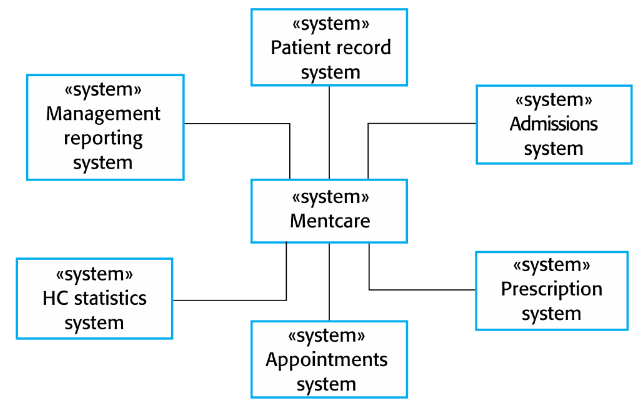
\includegraphics[width=0.5\textwidth]{images/context-mentcare-system.PNG}
    %\captionof{figure}{}
\end{minipage}

Il sistema Mentcare è collegato a un sistema di appuntamenti e a un sistema generale di archiviazione dei dati dei pazienti con cui condivide le informazioni. È inoltre connesso a sistemi per la reportistica gestionale, per le ammissioni ospedaliere e a un sistema statistico che raccoglie informazioni per la ricerca. Infine, utilizza un sistema di prescrizione per generare le ricette per i farmaci.
\end{Example}

I modelli di contesto mostrano semplicemente gli altri sistemi nell'ambiente, non come il sistema in fase di sviluppo viene utilizzato in quell'ambiente.

I modelli di contesto normalmente indicano che l'ambiente include diversi altri sistemi automatizzati, ma non mostrano i tipi di relazioni tra il sistema e quelli esterni. Pertanto, i modelli di contesto semplici vengono utilizzati insieme ad altri modelli, come i modelli di processo aziendale, che descrivono i processi umani e automatizzati in cui vengono utilizzati particolari sistemi software.

I diagrammi delle attività UML possono essere utilizzati per mostrare i processi aziendali in cui vengono utilizzati i sistemi. 

\begin{Example}{Modello di processo di detenzione involontaria}{}
\textit{La figura è un diagramma delle attività UML che illustra il processo di detenzione involontaria nell'assistenza sanitaria mentale, in cui viene utilizzato il sistema Mentcare.}

\begin{minipage}{\textwidth}
    \centering
    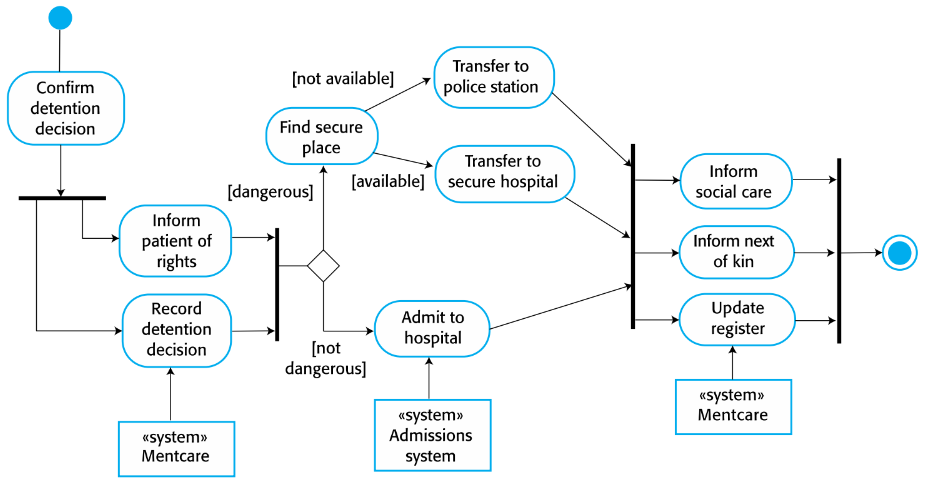
\includegraphics[width=0.7\textwidth]{images/process-model-involuntary-detention.PNG}
    %\captionof{figure}{}
\end{minipage}

%In alcuni casi, i pazienti con problemi di salute mentale possono rappresentare un pericolo per sé stessi o per gli altri. Potrebbe quindi essere necessario trattenerli in ospedale contro la loro volontà. La detenzione è soggetta a rigide garanzie legali; ad esempio, la decisione di trattenere un paziente deve essere rivista periodicamente. Una funzione critica del sistema Mentcare è garantire che queste garanzie siano rispettate e che i diritti dei pazienti siano protetti.
\end{Example}

I diagrammi delle attività UML mostrano le attività di un processo e il flusso di controllo da un'attività all'altra. L'inizio del processo è indicato da un cerchio pieno, la fine da un cerchio pieno all'interno di un altro cerchio. I rettangoli con angoli arrotondati rappresentano le attività, ovvero i sottoprocessi specifici che devono essere eseguiti.

Le frecce rappresentano il flusso di lavoro tra le attività, e una barra piena indica il coordinamento delle attività. Se il flusso di più attività porta a una barra piena, tutte queste attività devono essere completate prima che si possa proseguire. Quando il flusso da una barra piena conduce a diverse attività, queste possono essere eseguite in parallelo.

Le frecce possono essere annotate con guardie (tra parentesi quadre) che specificano quando quel flusso deve essere seguito.

\section{Modelli di interazione}
La modellazione dell'interazione utente è importante per identificare i requisiti dell'utente. La modellazione dell'interazione tra sistemi evidenzia i problemi di comunicazione che potrebbero sorgere. La modellazione dell'interazione tra componenti ci aiuta a capire se una struttura proposta per il sistema è in grado di garantire le prestazioni e l'affidabilità richieste. I  diagrammi dei casi d'uso e i diagrammi di sequenza possono essere utilizzati per la modellazione dell'interazione.

\subsection{Modellazione degli use case}
Ogni caso d'uso rappresenta un'attività specifica che comporta l'interazione con il sistema. Nella sua forma più semplice, un caso d'uso è rappresentato come un'ellisse, con gli attori coinvolti rappresentati come figure stilizzate.

\begin{Example}{Caso d'uso di trasferimento dati}{}
\textit{La figura mostra un caso d'uso per il sistema Mentcare, che rappresenta il compito di caricare i dati dal sistema Mentcare a un sistema generale di archiviazione dei dati dei pazienti, il quale mantiene i dati riassuntivi sui pazienti.}

\begin{minipage}{\textwidth}
    \centering
    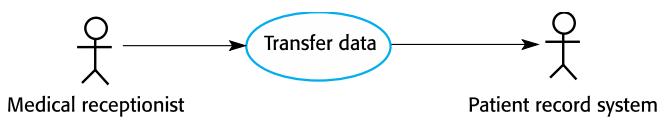
\includegraphics[width=0.5\textwidth]{images/transfer-data-use-case.PNG}
    %\captionof{figure}{}
\end{minipage}

I diagrammi dei casi d'uso forniscono una panoramica semplice dell'interazione, ma è necessario aggiungere maggiori dettagli per una descrizione completa.

\begin{minipage}{\textwidth}
\rowcolors{2}{lightblue}{lightgray}
\begin{tabular}{|p{3cm}|p{10.5cm}|}
\hline
\rowcolor{headerblue}
\textbf{\textcolor{white}{Caso d'Uso}} & \textbf{\textcolor{white}{MHC-PMS: Trasferimento dati}} \\\hline
Attori & Receptionist medico, sistema di registrazione pazienti (PRS)\\\hline
Descrizione & Un receptionist può trasferire dati dal sistema Mentcare a un database generale di registrazione pazienti gestito da un’autorità sanitaria. Le informazioni trasferite possono riguardare dati personali aggiornati (indirizzo, numero di telefono, ecc.) o un riepilogo della diagnosi e del trattamento del paziente.\\\hline
Dati & Informazioni personali del paziente, riepilogo del trattamento\\\hline
Stimolo & Comando dell'utente emesso dal receptionist medico\\\hline
Risposta & Conferma che il PRS è stato aggiornato\\\hline
Commenti & Il receptionist deve avere le autorizzazioni di sicurezza appropriate per accedere alle informazioni del paziente e al PRS.\\\hline
\end{tabular}
\end{minipage}
\vspace{.1cm}

I diagrammi di casi d'uso compositi mostrano più casi d'uso. A volte è possibile includere tutte le interazioni in un unico diagramma composito, ma, se il numero di casi d'uso è elevato, si possono sviluppare più diagrammi con casi d'uso correlati.

\begin{minipage}{\textwidth}
    \centering
    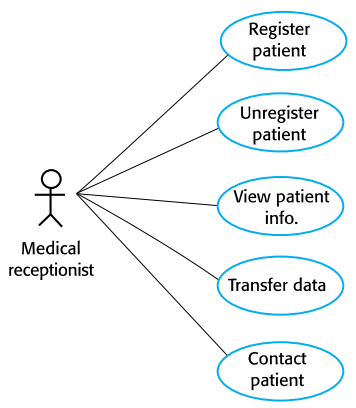
\includegraphics[width=0.35\textwidth]{images/use-case-mentcare-medical-receptionist.PNG}
    %\captionof{figure}{}
\end{minipage}
\end{Example}

\subsection{Diagrammi di sequenza}
I diagrammi di sequenza in UML vengono utilizzati principalmente per modellare le interazioni tra attori e oggetti in un sistema e le interazioni tra gli oggetti stessi. Come suggerisce il nome, un diagramma di sequenza mostra la sequenza delle interazioni che avvengono durante un particolare caso d'uso o istanza di caso d'uso. 

Gli oggetti e gli attori coinvolti sono elencati in alto, con una linea tratteggiata verticale che scende da ciascuno di essi. Le frecce annotate indicano le interazioni tra oggetti. Il rettangolo sulle linee tratteggiate rappresenta la "lifeline" dell'oggetto, ossia il periodo in cui l'oggetto è coinvolto nell'elaborazione. La sequenza delle interazioni si legge dall'alto verso il basso. Le annotazioni sulle frecce indicano le chiamate agli oggetti, i parametri e i valori di ritorno. Per denotare delle alternative, si può rappresentate da una casella denominata “alt” con le condizioni in parentesi quadre.

\begin{Example}{Diagramma di sequenza per visualizzare le informazioni del paziente}{}
\textit{Questo diagramma modella le interazioni coinvolte nel caso d'uso "Visualizza informazioni sul paziente", in cui un receptionist medico può visualizzare alcune informazioni del paziente.}

\begin{minipage}{\textwidth}
    \centering
    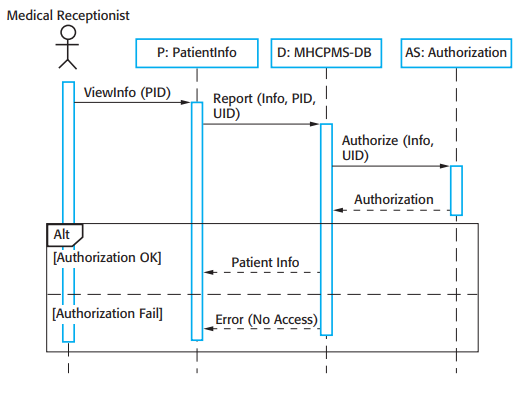
\includegraphics[width=0.6\textwidth]{images/sequence-diagram-view-patient-information.PNG}
    %\captionof{figure}{}
\end{minipage}

\begin{enumerate}
    \item Il \texttt{Medical Receptionist} attiva il metodo \texttt{ViewInfo} in un'istanza \texttt{P} della classe di oggetti \texttt{PatientInfo}, fornendo l'identificatore \texttt{PID} del paziente.
    \item L'istanza \texttt{P} interroga il database per ottenere le informazioni richieste.
    \item Il database verifica l'autorizzazione del receptionist tramite un sistema di autorizzazione.
    \item Se autorizzato, le informazioni del paziente vengono restituite e visualizzate sullo schermo; se l'autorizzazione fallisce, viene restituito un messaggio di errore.
\end{enumerate}
\end{Example}

\begin{Example}{Diagramma di sequenza per il trasferimento dei dati}{}
\textit{Viene creato un oggetto di tipo \texttt{Summary} per contenere i dati di riepilogo da caricare su un \texttt{PRS} (sistema di registrazione dei pazienti) nazionale.}

\begin{minipage}{\textwidth}
    \centering
    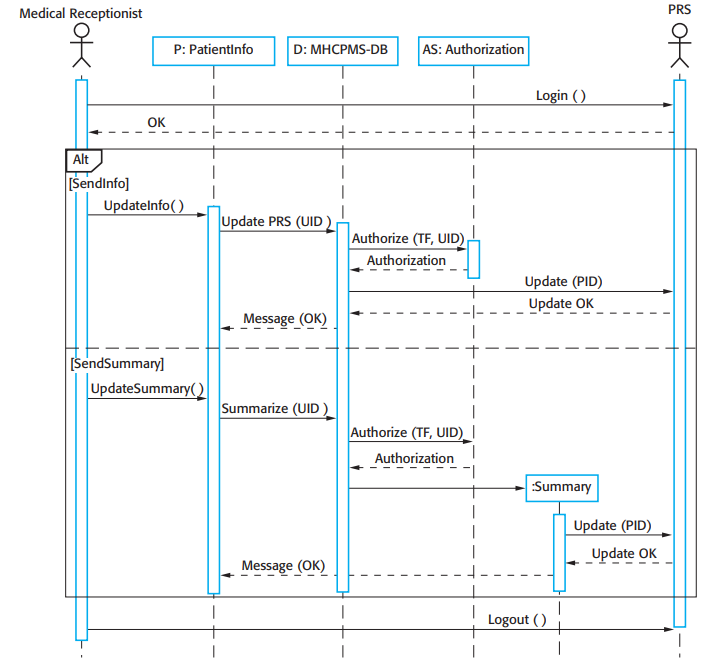
\includegraphics[width=0.8\textwidth]{images/sequence-diagram-transfer-data.PNG}
    %\captionof{figure}{}
\end{minipage}

\begin{enumerate}
    \item Il \texttt{Receptionist} accede al \texttt{PRS}.
    \item Sono disponibili due opzioni (come mostrato nel riquadro “alt”): il trasferimento diretto delle informazioni aggiornate del paziente dal database \texttt{Mentcare} al \texttt{PRS} e il trasferimento dei dati riepilogativi della salute dal database \texttt{Mentcare} al \texttt{PRS}.
    \item In ciascun caso, le autorizzazioni del receptionist vengono verificate utilizzando il sistema di autorizzazione.
    \item Le informazioni personali possono essere trasferite direttamente dall’oggetto dell’interfaccia utente al \texttt{PRS}. In alternativa, può essere creato un record riepilogativo dal database e quindi trasferito.
    \item Al termine del trasferimento, il \texttt{PRS} emette un messaggio di stato e l’utente effettua il logout.   
\end{enumerate} 
\end{Example}

\section{Modelli strutturali}
I modelli strutturali del software mostrano l'organizzazione di un sistema in termini di componenti che lo costituiscono e le loro relazioni. I modelli strutturali possono essere modelli statici, che mostrano l'organizzazione del progetto del sistema, o modelli dinamici, che mostrano l'organizzazione del sistema durante l'esecuzione.

Si creano modelli strutturali di un sistema durante la discussione e progettazione dell'architettura del sistema stesso.

\subsection{Diagrammi delle classi}
I diagrammi delle classi vengono utilizzati nello sviluppo di un modello orientato agli oggetti per mostrare le classi di un sistema e le associazioni tra queste classi. Una classe di oggetti può essere pensata come una definizione generale di un tipo di oggetto del sistema. Un'associazione è un collegamento tra classi che indica l'esistenza di una relazione tra di esse.

Durante la modellazione nelle prime fasi del processo di ingegneria del software, gli oggetti rappresentano qualcosa nel mondo reale, come un paziente, una prescrizione o un medico.

\begin{figure}[ht]
    \centering
    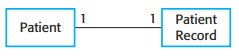
\includegraphics[width=0.25\linewidth]{images/uml-classes-association.PNG}
    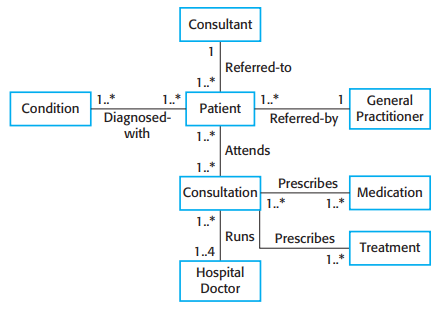
\includegraphics[width=0.51\linewidth]{images/classes-association-mhc-pms.PNG}
    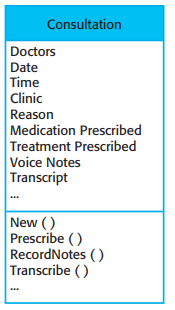
\includegraphics[width=0.22\linewidth]{images/consultation-class.PNG}
    \caption{Classi e associazioni UML}
    \label{fig:uml-classes-association}
\end{figure}

Una caratteristica importante dei diagrammi delle classi è la capacità di mostrare quanti oggetti sono coinvolti in un'associazione. Ciascuna estremità dell'associazione è annotata con un “1”, che significa che esiste una relazione 1:1 tra gli oggetti di queste classi. Cioè, ad esempio, ogni paziente ha esattamente un record e ogni record mantiene informazioni su un solo paziente.
Sono possibili anche altre molteplicità, ad esempio "*", indica che è presente un numero indefinito di oggetti nell'associazione. Ad esempio, la molteplicità (1..) nella relazione tra \texttt{Patient} e \texttt{Condition} mostra che un paziente può soffrire di più condizioni e che la stessa condizione può essere associata a più pazienti.

Per definire gli oggetti in modo più dettagliato, si aggiungono informazioni sui loro attributi (le caratteristiche dell'oggetto) e sulle operazioni (le funzioni dell'oggetto).

\subsection{Generalizzazione}
La generalizzazione è una tecnica quotidiana che utilizziamo per gestire la complessità. Anziché imparare le caratteristiche dettagliate di tutto ciò che incontriamo, apprendiamo classi generali (animali, automobili, case, ecc.) e le caratteristiche di queste classi. In seguito, riutilizziamo la conoscenza classificando gli oggetti e ci concentriamo sulle differenze tra essi e la loro classe. Ad esempio, gli scoiattoli e i ratti appartengono alla classe dei “roditori” e condividono quindi le caratteristiche dei roditori. Le affermazioni generali si applicano a tutti i membri della classe; ad esempio, tutti i roditori hanno denti per rosicchiare.

Quando si modellano sistemi, è spesso utile esaminare le classi in un sistema per verificare se esiste spazio per una generalizzazione e la creazione di classi. Questa è una buona pratica di progettazione, poiché significa che, se vengono proposte modifiche, non è necessario esaminare tutte le classi del sistema per vedere se sono influenzate dalla modifica. Nei linguaggi orientati agli oggetti, come Java, la generalizzazione viene implementata utilizzando i meccanismi di ereditarietà delle classi integrati nel linguaggio.

In una generalizzazione, gli attributi e le operazioni associati alle classi di livello superiore sono anche associati alle classi di livello inferiore. Le classi di livello inferiore sono sottoclassi che ereditano gli attributi e le operazioni dalle loro superclassi, alle quali aggiungono attributi e operazioni più specifici.

In UML la generalizzazione è mostrata con una freccia che punta verso l'alto alla classe più generale. 

\begin{figure}[ht]
    \centering
    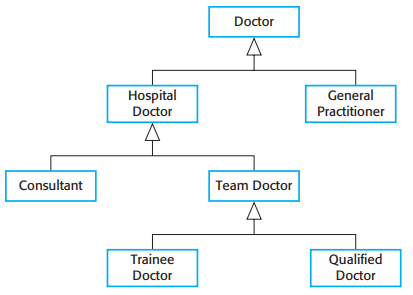
\includegraphics[width=0.45\linewidth]{images/generalizazion-hierarchy.PNG}
    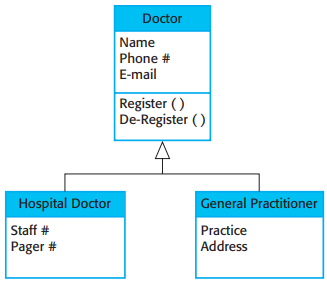
\includegraphics[width=0.37\linewidth]{images/generalizazion-hierarchy-detail.PNG}
    \caption{Gerarchia di generalizzazione}
    \label{fig:generalizazion-hierarchy}
\end{figure}

\subsection{Aggregazione}
L'UML fornisce un tipo speciale di associazione tra classi chiamato aggregazione, che indica che un oggetto (il tutto) è composto da altri oggetti (le parti). Per definire l'aggregazione, si aggiunge un rombo accanto al collegamento che rappresenta la classe che costituisce il tutto.

\begin{figure}[ht]
    \centering
    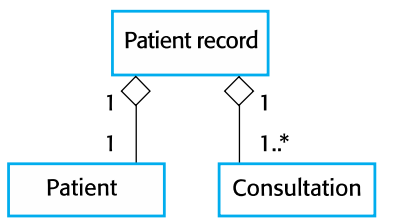
\includegraphics[width=0.3\linewidth]{images/aggregation-association.PNG}
    \caption{Associazione di aggregazione}
    \label{fig:aggregation-association}
\end{figure}

\section{Modelli comportamentali}
I modelli comportamentali sono rappresentazioni del comportamento dinamico di un sistema durante la sua esecuzione. Mostrano cosa accade o dovrebbe accadere quando un sistema risponde a uno stimolo proveniente dall’ambiente esterno. Questi stimoli possono essere dati o eventi:
\begin{enumerate}
    \item I dati diventano disponibili e devono essere elaborati dal sistema.
    \item Si verifica un evento che attiva l'elaborazione del sistema. Gli eventi possono avere dati associati, anche se non sempre è così.
\end{enumerate}

\subsection{Modelli guidati dai dati}
Molti sistemi aziendali sono sistemi di elaborazione dati, guidati principalmente dai dati stessi. Sono controllati dall’input di dati fornito al sistema e presentano relativamente pochi eventi esterni.

I modelli guidati dai dati mostrano la sequenza di azioni coinvolte nell’elaborazione dei dati di input e nella generazione di un output associato. Possono essere utilizzati durante l'analisi dei requisiti, poiché mostrano l'elaborazione end-to-end in un sistema. Ovvero, rappresentano l'intera sequenza di azioni che avviene dall'inizio dell'elaborazione di un input fino all'output corrispondente, che rappresenta la risposta del sistema.

I diagrammi di flusso dei dati possono essere rappresentati in UML utilizzando i diagrammi di attività. I passaggi di elaborazione, rappresentati come attività (rettangoli con angoli arrotondati), e i dati che fluiscono tra questi passaggi, rappresentati come oggetti (rettangoli).

\begin{figure}[ht]
    \centering
    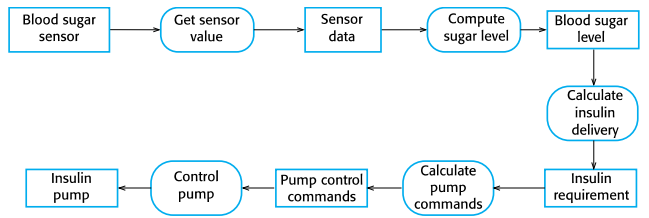
\includegraphics[width=0.65\linewidth]{images/activity-model-insulin-pump-operation.PNG}
    \caption{Modello di attività del funzionamento della pompa per insulina}
    \label{fig:activity-model-insulin-pump-operation}
\end{figure}

Un’alternativa per mostrare la sequenza di elaborazione in un sistema è utilizzare i diagrammi di sequenza UML. Abbiamo già visto come questi diagrammi possano essere usati per modellare le interazioni, ma se li si disegna in modo che i messaggi siano inviati solo da sinistra a destra, mostrano la sequenza di elaborazione dei dati nel sistema. 

\begin{figure}[ht]
    \centering
    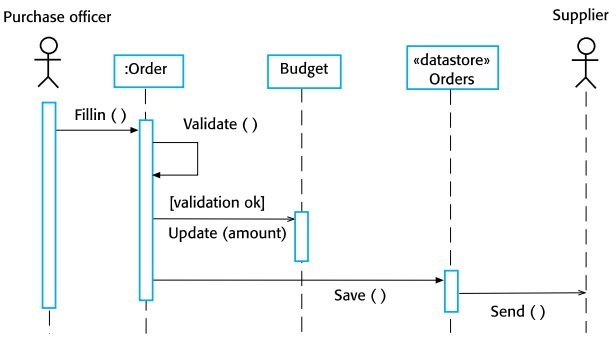
\includegraphics[width=0.6\linewidth]{images/order-processing.PNG}
    \caption{Elaborazione degli ordini}
    \label{fig:order-processing}
\end{figure}

\subsection{Modelli guidati dagli eventi}
I sistemi in tempo reale sono solitamente guidati dagli eventi, con una limitata elaborazione dei dati. Ad esempio, un sistema di commutazione telefonica risponde ad eventi come "ricevitore sollevato" generando un segnale di linea libera.

La modellazione guidata dagli eventi mostra come un sistema risponde a eventi esterni e interni. Si basa sull'assunzione che un sistema abbia un numero finito di stati e che gli eventi (stimoli) possano causare una transizione da uno stato all'altro.

L’UML supporta la modellazione basata sugli eventi mediante diagrammi di stato, basati sugli Statechart. I diagrammi di stato mostrano gli stati del sistema e gli eventi che causano le transizioni da uno stato all’altro.

Nei diagrammi di stato UML, i rettangoli con angoli arrotondati rappresentano gli stati del sistema. Possono includere una breve descrizione (dopo la parola "do") delle azioni eseguite in quello stato. Le frecce etichettate rappresentano gli stimoli che forzano una transizione da uno stato all'altro. È possibile indicare gli stati di inizio e fine con cerchi pieni, come nei diagrammi di attività.

\begin{Example}{Diagramma di stato di un forno a microonde}{}
\textit{Per illustrare la modellazione guidata dagli eventi, utilizzo un esempio di software di controllo per un forno a microonde molto semplice. }

\begin{minipage}{\textwidth}
    \centering
    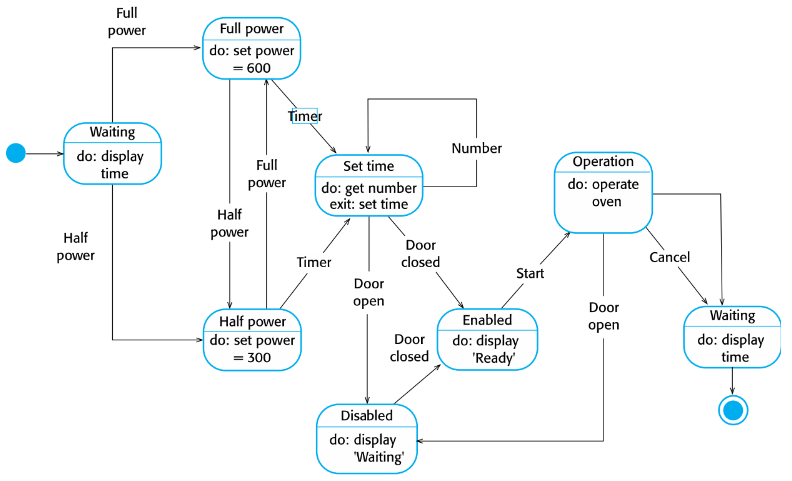
\includegraphics[width=0.8\textwidth]{images/state-diagram-microwave-oven.PNG}
    %\captionof{figure}{}
\end{minipage}

Questo forno semplice ha un interruttore per selezionare potenza massima o ridotta, una tastiera numerica per impostare il tempo di cottura, un pulsante di avvio/arresto e un display alfanumerico.

Si presume che la sequenza di azioni per l’uso del microonde sia la seguente:
\begin{enumerate}
    \item Selezionare il livello di potenza (metà potenza o potenza massima).
    \item Impostare il tempo di cottura utilizzando una tastiera numerica.
    \item Premere Avvio e il cibo viene cotto per il tempo impostato.
\end{enumerate}
Per motivi di sicurezza, il forno non dovrebbe funzionare quando la porta è aperta e, al termine della cottura, viene emesso un segnale acustico. Il forno ha un semplice display utilizzato per visualizzare vari avvisi e messaggi di allarme.

Si può vedere che il sistema parte in uno stato di attesa e risponde inizialmente a uno dei pulsanti di selezione della potenza. Gli utenti possono cambiare idea dopo aver selezionato uno di questi pulsanti e possono premere l’altro. Viene impostato il tempo e, se la porta è chiusa, il pulsante di avvio è abilitato. Premendo questo pulsante inizia l'operazione del forno, che cucina per il tempo specificato. Questo è il termine del ciclo di cottura e il sistema ritorna allo stato di attesa.

Il problema con la modellazione basata sugli stati è che il numero di stati possibili aumenta rapidamente. Per i modelli di grandi dimensioni, quindi, è necessario nascondere i dettagli nei modelli. Un modo per farlo è utilizzare il concetto di superstato che incapsula una serie di stati separati. 

\begin{minipage}{\textwidth}
    \centering
    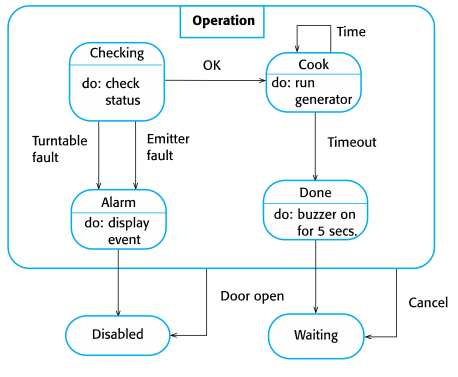
\includegraphics[width=0.5\textwidth]{images/microwave-oven-operation.PNG}
    %\captionof{figure}{}
\end{minipage}

Lo stato di Operazione include una serie di sottostati. Mostra che l'operazione inizia con un controllo di stato e che, se vengono rilevati problemi, viene attivato un allarme e l'operazione viene disabilitata. La cottura implica l'attivazione del generatore a microonde per il tempo specificato; al termine, viene emesso un segnale acustico. Se la porta viene aperta durante l'operazione, il sistema passa allo stato di disabilitazione.

I modelli a stati di un sistema forniscono una panoramica dell'elaborazione degli eventi, ma normalmente è necessario estenderli con una descrizione più dettagliata degli stimoli e degli stati del sistema.

\vspace{0.1cm}
\begin{minipage}{\textwidth}
\rowcolors{2}{lightblue}{lightgray}
\begin{tabular}{|p{3cm}|p{10.5cm}|}
\hline
\rowcolor{headerblue}
\textbf{\textcolor{white}{Stato}} & \textbf{\textcolor{white}{Descrizione}} \\\hline
Attesa & Il forno è in attesa di input. Il display mostra l’ora corrente.\\\hline
Mezza potenza & La potenza del forno è impostata a 300 watt. Il display mostra ‘Mezza potenza’.\\\hline
Potenza massima & La potenza del forno è impostata a 600 watt. Il display mostra ‘Potenza massima’.\\\hline
Imposta tempo & Il tempo di cottura è impostato al valore inserito dall’utente. Il display mostra il tempo di cottura selezionato e viene aggiornato mentre il tempo viene impostato.\\\hline
Disabilitato & Il funzionamento del forno è disabilitato per sicurezza. La luce interna del forno è accesa. Il display mostra ‘Non pronto’.\\\hline
Abilitato & Il funzionamento del forno è abilitato. La luce interna del forno è spenta. Il display mostra ‘Pronto per la cottura’.\\\hline
Operazione & Il forno è in funzione. La luce interna del forno è accesa. Il display mostra il conto alla rovescia del timer. Al termine della cottura, il segnale acustico suona per cinque secondi. La luce del forno è accesa. Il display mostra ‘Cottura completata’ mentre il segnale acustico è attivo.\\\hline
\end{tabular}
\end{minipage}

\vspace{0.1cm}
\begin{minipage}{\textwidth}
\rowcolors{2}{lightblue}{lightgray}
\begin{tabular}{|p{3cm}|p{10.5cm}|}
\hline
\rowcolor{headerblue}
\textbf{\textcolor{white}{Stimolo}} & \textbf{\textcolor{white}{Descrizione}} \\\hline
Mezza potenza & L'utente ha premuto il pulsante per la mezza potenza.\\\hline
Potenza massima & L'utente ha premuto il pulsante per la potenza massima.\\\hline
Timer & L'utente ha premuto uno dei pulsanti del timer.\\\hline
Numero & L'utente ha premuto un tasto numerico.\\\hline
Porta aperta & L'interruttore della porta del forno non è chiuso.\\\hline
Porta chiusa & L'interruttore della porta del forno è chiuso.\\\hline
Avvio & L'utente ha premuto il pulsante Avvio.\\\hline
Annulla & L'utente ha premuto il pulsante Annulla.\\\hline
\end{tabular}
\end{minipage}
\end{Example}


\section{Ingegneria guidata dai modelli}
L’ingegneria guidata dai modelli (MDE, Model-Driven Engineering) è un approccio allo sviluppo software in cui i modelli, piuttosto che i programmi, sono i principali risultati del processo di sviluppo. I programmi che vengono eseguiti su una piattaforma hardware/software vengono generati automaticamente a partire dai modelli. I sostenitori della MDE sostengono che questo innalza il livello di astrazione nell'ingegneria del software, così che gli ingegneri non devono più preoccuparsi dei dettagli del linguaggio di programmazione o delle specificità delle piattaforme di esecuzione.

L'ingegneria guidata da modelli è ancora in una fase iniziale di sviluppo, ed è incerto se avrà o meno un effetto significativo sulla pratica dell'ingegneria del software. Da un lato permette di considerare i sistemi a livelli di astrazione più alti e di generare codice automaticamente in modo da rendere meno costoso adattare i sistemi a nuove piattaforme; dall'altro i modelli per l'astrazione non sono necessariamente adatti all'implementazione e i risparmi derivanti dalla generazione automatica di codice possono essere superati dai costi di sviluppo dei traduttori per nuove piattaforme.

\subsection{Architettura guidata da modelli}
L'architettura guidata da modelli (Model-Driven Architecture o MDA) è un approccio alla progettazione e implementazione del software che si focalizza sui modelli e utilizza un sottoinsieme di modelli UML per descrivere un sistema. In questo approccio vengono creati modelli a diversi livelli di astrazione. Da un modello indipendente dalla piattaforma di alto livello è possibile, in teoria, generare un programma funzionante senza intervento manuale.

Il metodo MDA consiglia la produzione di tre tipi di modelli astratti del sistema:
\begin{enumerate}
    \item \textit{Modello indipendente dal calcolo (Computation Independent Model o CIM)}.
    I CIM rappresentano le astrazioni dominanti importanti utilizzate in un sistema e sono a volte chiamati modelli di dominio.
    \item \textit{Modello indipendente dalla piattaforma (Platform-Independent Model o PIM)}.
    I PIM rappresentano il funzionamento del sistema senza riferimenti alla sua implementazione. Di solito, un PIM è descritto usando modelli UML che mostrano la struttura statica del sistema e il modo in cui risponde a eventi esterni e interni.
    \item \textit{Modelli specifici della piattaforma (Platform-Specific Models o PSM)}.
    I PSM sono trasformazioni del modello indipendente dalla piattaforma con un PSM separato per ogni piattaforma applicativa. In teoria, potrebbero esserci livelli di PSM, con ogni livello che aggiunge qualche dettaglio specifico della piattaforma.
\end{enumerate}
Il concetto fondamentale di MDA è che le trasformazioni tra modelli possono essere definite e applicate automaticamente tramite strumenti software, come illustrato nella Figura \ref{fig:mda-transformations}. Questo diagramma mostra anche un livello finale di trasformazione automatica in cui una trasformazione è applicata al PSM per generare il codice eseguibile che verrà eseguito sulla piattaforma software designata.

\begin{figure}[ht]
    \centering
    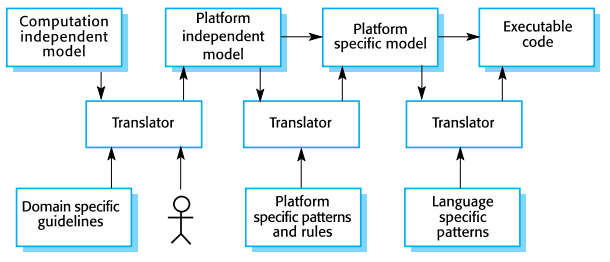
\includegraphics[width=0.55\linewidth]{images/mda-transformations.PNG}
    \caption{Trasformazioni MDA}
    \label{fig:mda-transformations}
\end{figure}

La traduzione da modelli indipendenti dalla piattaforma a modelli specifici della piattaforma è un problema tecnico più semplice. Esistono strumenti commerciali e open-source che forniscono traduttori dai PIM a piattaforme comuni come Java e J2EE. Potrebbero esserci diversi PSM per ogni PIM nel sistema. Se un sistema software è destinato a funzionare su piattaforme diverse (ad es., J2EE e .NET), allora, in teoria, è sufficiente mantenere un unico PIM. I PSM per ciascuna piattaforma sono generati automaticamente (Figura \ref{fig:multple-platform-specific-models}).

\begin{figure}[ht]
    \centering
    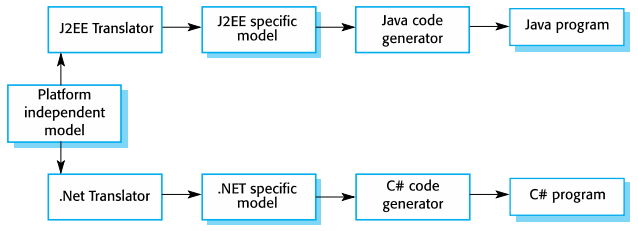
\includegraphics[width=0.6\linewidth]{images/multple-platform-specific-models.PNG}
    \caption{Modelli multipli specifici per piattaforma}
    \label{fig:multple-platform-specific-models}
\end{figure}

Ritengo che ci siano diversi altri motivi per cui MDA non è diventato un approccio di riferimento nello sviluppo software:
\begin{enumerate}
    \item I modelli sono un buon modo per facilitare le discussioni su una progettazione software. Tuttavia, ciò non implica sempre che le astrazioni utili per le discussioni siano le astrazioni giuste per l'implementazione.
    \item Per la maggior parte dei sistemi complessi, l'implementazione non è il problema principale: l'ingegneria dei requisiti, la sicurezza e l'affidabilità, l'integrazione con i sistemi legacy e i test sono tutti aspetti più significativi.
    \item Gli argomenti per l'indipendenza dalla piattaforma sono validi solo per sistemi di grandi dimensioni e di lunga durata. Per i prodotti software e i sistemi informativi sviluppati per piattaforme standard i risparmi derivanti dall'uso di MDA potrebbero essere superati dai costi di introduzione e di configurazione.
    \item La diffusione dei metodi agili nello stesso periodo in cui MDA si stava sviluppando ha distolto l'attenzione dagli approcci guidati da modelli.
\end{enumerate}
I casi di successo per MDA provengono principalmente da aziende che sviluppano prodotti di sistema, che includono sia hardware che software. Il software in questi prodotti ha una lunga durata e potrebbe dover essere modificato per riflettere i cambiamenti delle tecnologie hardware.

Esiste una relazione difficile tra metodi agili e architettura guidata da modelli. L'idea di una modellazione preliminare estesa contraddice i principi fondamentali del manifesto agile e sospetto che pochi sviluppatori agili si sentano a proprio agio con l'ingegneria guidata da modelli.

\newpage
\section{Punti chiave}
\begin{center}
\begin{minipage}{\textwidth}
\colorbox{lightgray}{
\parbox{\linewidth}{
\begin{itemize} 
    \item Un modello è una rappresentazione astratta di un sistema che ignora i dettagli specifici. È possibile sviluppare modelli complementari del sistema per mostrare il contesto, le interazioni, la struttura e il comportamento del sistema.
    \item I modelli di contesto mostrano come un sistema in fase di modellazione sia posizionato in un ambiente con altri sistemi e processi.
    \item I diagrammi dei casi d’uso e i diagrammi di sequenza vengono utilizzati per descrivere le interazioni tra utenti e sistemi in fase di progettazione. I casi d'uso descrivono le interazioni tra un sistema e gli attori esterni; i diagrammi di sequenza aggiungono ulteriori informazioni mostrando le interazioni tra gli oggetti del sistema.
    \item I modelli strutturali mostrano l’organizzazione e l’architettura di un sistema. I diagrammi delle classi sono utilizzati per definire la struttura statica delle classi in un sistema e le loro associazioni.
    \item I modelli comportamentali sono usati per descrivere il comportamento dinamico di un sistema in esecuzione. Questo comportamento può essere modellato dalla prospettiva dei dati elaborati dal sistema o dagli eventi che stimolano le risposte del sistema.
    \item I diagrammi di attività possono essere usati per modellare l'elaborazione dei dati, dove ogni attività rappresenta un passaggio del processo.
    \item I diagrammi di stato sono utilizzati per modellare il comportamento di un sistema in risposta a eventi interni o esterni.
    \item L'ingegneria guidata da modelli è un approccio allo sviluppo software in cui un sistema è rappresentato come un insieme di modelli che possono essere automaticamente trasformati in codice eseguibile.
\end{itemize}
}}
\end{minipage}
\end{center}